\chapter{Combinatorial Factor}\label{app:combinatorial factor}
        The easiest way to calculate the required combinatorial factor is diagrammatic.
        We start with
        \begin{equation}
            I = \int \!\! \dl{t} \int \!\! \dl{t'} J(t) \Delta(t, t') J(t') = 
            \tikzsetnextfilename{combinatorial-factor-1}
            \begin{tikzpicture}[baseline=-0.08cm]
                \draw (0, 0) -- (1, 0);
                \node at (0, 0) {\(\times\)};
                \node at (1, 0) {\(\times\)};
            \end{tikzpicture}
        \end{equation}
        The two ends correspond to the two times, \(t\) and \(t'\), at which \(J\) is evaluated and the line between to the propagator \(\Delta(t, t')\).
        We then write
        \begin{equation}
            \diffd{}{J(\tau)}I = \diffd{}{J(\tau)} \int J(t) \Delta(t, t') J(t') \dd{t} = \int \!\! \dl{t'} \Delta(\tau, t')J(t') =
            \tikzsetnextfilename{combinatorial-factor-2}
            \begin{tikzpicture}[baseline=-0.1cm]
                \draw (0, 0) -- (1, 0);
                \fill (0, 0) circle [radius = 0.05] node[above] {\(\tau\)};
                \node at (1, 0) {\(\times\)};
            \end{tikzpicture}
        \end{equation}
        
        For the four-point correlation function we are then considering terms with
        \begin{equation}
            I^4 = 
            \tikzsetnextfilename{combinatorial-factor-3}
            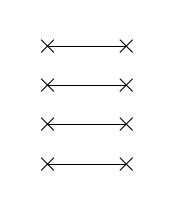
\begin{tikzpicture}[baseline=0.7cm]
                \foreach \y in {0, 0.5, 1, 1.5} {
                    \draw (0, \y) -- (1, \y);
                    \node at (0, \y) {\(\times\)};
                    \node at (1, \y) {\(\times\)};
                }
            \end{tikzpicture}
        \end{equation}
        We then act on this with the derivative
        \begin{equation}
            \diffd{}{J(t_1),J(t_2),J(t_3),J(t_4)} \diffd[4]{}{J(\tau)}.
        \end{equation}
        When doing the derivatives with respect to \(J(\tau)\) we want to consider only the terms where each derivative acts on a \(J\) from a different term.
        This gives the connected term.
        We also want to account for the number of ways we can do this, which is where the combinatorial argument comes in.
        First we need to choose one of the terms to act on with the first \(J(\tau)\) derivative, as well as one of the ends, there are obviously \(8\) choices here, since there are 8 ends.
        Without loss of generality we choose the bottom right giving
        \begin{equation}
            \diffd[4]{}{J(\tau)} I^4 = 8\diffd[3]{}{J(\tau)}
            \tikzsetnextfilename{combinatorial-factor-4}
            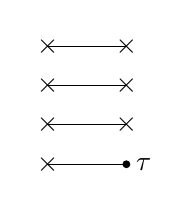
\begin{tikzpicture}[baseline=0.7cm]
                \foreach \y in {0, 0.5, 1, 1.5} {
                    \draw (0, \y) -- (1, \y);
                    \node at (0, \y) {\(\times\)};
                }
                \fill (1, 0) circle [radius = 0.05] node[right] {\(\tau\)};
                \foreach \y in {0.5, 1, 1.5} {\node at (1, \y) {\(\times\)};}
            \end{tikzpicture}
        \end{equation}
        For the next derivative since we want to act on a term that we haven't used yet, ruling out the bottom term, we have \(6\) choices.
        Without loss of generality we choose the second bottom right giving
        \begin{equation}
            \diffd[4]{}{J(\tau)} I^4 = 8 \cdot 6 \diffd[2]{}{J(\tau)}
            \tikzsetnextfilename{combinatorial-factor-5}
            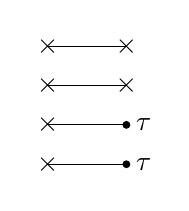
\begin{tikzpicture}[baseline=0.7cm]
                \foreach \y in {0, 0.5, 1, 1.5} {
                    \draw (0, \y) -- (1, \y);
                    \node at (0, \y) {\(\times\)};
                }
                \fill (1, 0) circle [radius = 0.05] node[right] {\(\tau\)};
                \fill (1, 0.5) circle [radius = 0.05] node[right] {\(\tau\)};
                \foreach \y in {1, 1.5} {\node at (1, \y) {\(\times\)};}
            \end{tikzpicture}
        \end{equation}
        The next two choices proceed similarly with \(4\) and then \(2\) options, making these choices we have, without loss of generality,
        \begin{equation}
            \diffd[4]{}{J(\tau)} I^4 = 8 \cdot 6 \cdot 4 \cdot 2 
            \tikzsetnextfilename{combinatorial-factor-6}
            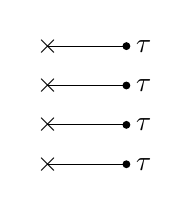
\begin{tikzpicture}[baseline=0.7cm]
                \foreach \y in {0, 0.5, 1, 1.5} {
                    \draw (0, \y) -- (1, \y);
                    \node at (0, \y) {\(\times\)};
                    \fill (1, \y) circle [radius = 0.05] node[right] {\(\tau\)};
                }
            \end{tikzpicture}
        \end{equation}
        Note that
        \begin{equation}
            8 \cdot 6 \cdot 4 \cdot 2 = 2^44!.
        \end{equation}
        
        Next we have to compute the derivatives with respect to \(J(t_i)\).
        First for \(J(t_i)\) there are 4 options, without loss of generality we first compute the derivative with respect to \(J(t_4)\) giving
        \begin{equation*}
            \diffd{}{J(t_1),J(t_2),J(t_3),J(t_4)}\diffd[4]{}{J(\tau)} I^4 = 3 \cdot 2^44! \diffd{}{J(t_1),J(t_2),J(t_3)}
            \tikzsetnextfilename{combinatorial-factor-7}
            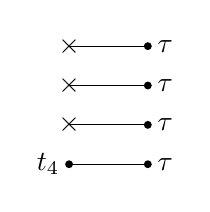
\begin{tikzpicture}[baseline=0.7cm]
                \foreach \y in {0, 0.5, 1, 1.5} {
                    \draw (0, \y) -- (1, \y);
                    \fill (1, \y) circle [radius = 0.05] node[right] {\(\tau\)};
                }
                \foreach \y in {0.5, 1, 1.5} {\node at (0, \y) {\(\times\)};}
                \fill (0, 0) circle [radius = 0.05] node[left] {\(t_4\)};
            \end{tikzpicture}
        \end{equation*}
        There are then \(3\) choices for the derivative with respect to \(J(t_3)\), \(2\) choices for the derivative with respect to \(J(t_2)\), and \(1\) choice for the derivative with respect to \(J(t_1)\).
        This gives another factor of \(4!\):
        \begin{equation}
            \diffd{}{J(t_1),J(t_2),J(t_3),J(t_4)}\diffd[4]{}{J(\tau)} I^4 = 2^4(4!)^2
            \tikzsetnextfilename{combinatorial-factor-8}
            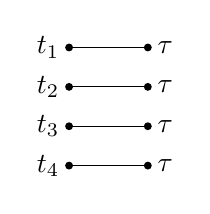
\begin{tikzpicture}[baseline=0.7cm]
                \foreach \y in {0, 0.5, 1, 1.5} {
                    \draw (0, \y) -- (1, \y);
                    \fill (1, \y) circle [radius = 0.05] node[right] {\(\tau\)};
                    \fill (0, \y) circle [radius = 0.05] node[left] {\(t_{\pgfmathparse{int(4 - 2*\y)}\pgfmathresult}\)};
                }
            \end{tikzpicture}
        \end{equation}
        
        Finally noticing that four points correspond to \(\tau\) we can simplify the diagram to be
        \begin{equation}
            \diffd{}{J(t_1),J(t_2),J(t_3),J(t_4)}\diffd[4]{}{J(\tau)} I^4 = 2^4(4!)^2
            \tikzsetnextfilename{combinatorial-factor-9}
            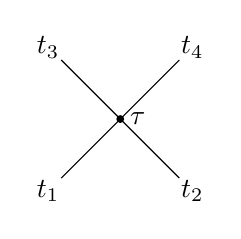
\begin{tikzpicture}[baseline=0.75cm]
                \draw (0, 0) -- (1.5, 1.5);
                \draw (0, 1.5) -- (1.5, 0);
                \fill (0.75, 0.75) circle [radius = 0.05] node[right] {\(\tau\)};
                \node[below left] at (0.1, 0.1) {\(t_1\)};
                \node[above left] at (0.1, 1.4) {\(t_3\)};
                \node[below right] at (1.4, 0.1) {\(t_2\)};
                \node[above right] at (1.4, 1.4) {\(t_4\)};
            \end{tikzpicture}
        \end{equation}
        We can then use the Feynman rules to recover the result.